\documentclass[12pt,a4paper]{article}
\usepackage[latin1]{inputenc}
\usepackage{amsmath}
\usepackage{amsfonts}
\usepackage{amssymb}
\usepackage{graphicx}
\author{Emanuele Varriale}
\title{Notes on clique encoding networks}
\usepackage[backend=bibtex]{biblatex}
\bibliography{bibliography}
\begin{document}
	\maketitle
	\section{Introduction}
		The brain typically shows robust internal activity which is only modulated, but not driven, by sensory input, as the activity persists even in absence of such an input \cite{fiser_small_2004}. One could then wonder how does the internal dynamics relate to the sensory input and, in particular, how does meaning from the outside world get represented by network activity. 
		
		One possibility is to consider networks with transient state dynamics, i.e.\ networks whose activity consists of a series of attractor states, which are only transiently stable \cite{gros_semantic_2010}. Importantly, the attractor states themselves  are inherent to the network structure, and are not a product of external input. Such a network can be built as a collection of cliques, i.e.\ fully connected sub-networks. Connections  within cliques are only excitatory whereas among cliques they are mostly inhibitory, so that the network behaves in a multi-winner-take-all fashion. 
		
		The external input can then make use of pre-existing attractor states, acting as a bifurcation parameter, and confer semantic content to the network with a suitable learning rule that correlates input data to transient attractor dynamics. 
		
		We present a study on the internal transient state dynamics of networks with different architectures and, furthermore, we couple the network with an external input, from the bars problem, and analyse the resulting dynamics.
		
	\section{The network}
	\subsection{Architecture}
		Let's start by describing the possible network architectures for clique encoding. For simplicity we use undirected graph (i.e. symmetrical synapses) and neurons that have both excitatory and inhibitory synapses.
			
		One could build an Erd\"{o}s-Renyi kind of graph with excitatory connections and then complete the graph with inhibitory ones. This approach would lead to random cliques with an irregular autonomous dynamics, thus making even harder the search for a learning rule that couple cliques to sensory input.
			
		We have therefore worked with more regular networks which are described by the number of cliques $n_c$ and their size $s_c$. Each clique is a complete sub-graph with excitatory connections, and inhibitory connections exist only among different cliques. We worked with two kinds of networks which we named \emph{geometric} and \emph{rotating}, two examples are shown in Fig. \ref{fig:network}. 
		
		In the geometric arrangement each clique has two neurons that have an excitatory connection with another clique, while in the rotating arrangement every neuron of each clique has one such connection; but in both cases each clique can excite two other cliques. 
		
		The inhibitory connections either complete the graph, or are drawn with a probability P such that the average number of inhibitory synapses is equal to the number of excitatory ones.
		
		We will focus on the \emph{rotating} network.
		\begin{figure}
			\centering
			\includegraphics[width=0.45\linewidth]{../geometric/4x3net_r}
			\includegraphics[width=0.45\linewidth]{../rotating/4x3_sFalse.png}
			\caption{Left: a geometric network with $n_c = 3$ and $s_c = 3$. Right: a rotating network with $n_c = 3$ and $s_c = 4$.}
			\label{fig:network}
		\end{figure}
		
	\subsection{Weights}
		We choose the weights so that the input approximately lies in the range $[-1, \, 1]$. The activation function of neurons is a sigmoidal whose output is restricted to $[0, \, 1]$. To have the transient state dynamics we need high input for neurons belonging to the winning clique and negative input for those outside.
		We call the excitatory weights $w_{jk}$ and the inhibitory $z_{jk}$, $w_{jk}^{\text{inter}}$ are inter-clique excitatory connections.
		
		Let's consider then, respectively, neurons in the winning clique, and in the losing cliques only with negative inputs:
		\begin{equation}
			x_{\text{inp}} = \sum_{i=1}^{s_c - 1} w_{jk} y \approx \left(s_c -1 \right) \bar{w} \approx 1 \implies \bar{w} = \frac{1}{s_c - 1 }
		\end{equation}
		\begin{equation}
		x_{\text{inp}} = \sum_{i=1}^{s_c} z_{jk} y \approx s_c \bar{z} \approx -1 \implies \bar{z} = -\frac{1}{s_c}
		\end{equation}
		and for the inter-clique excitatory connections the input will be inevitably larger than the last case, for similarity with the above formulas, we choose 
		\begin{equation}
			w_{jk}^{\text{inter}} = \frac{1}{s_c} \implies x_{\text{inp}} \approx (s_c -1) \bar{z} +  \bar{w}^{\text{inter}} = -1 +\frac{2}{s_c}.
		\end{equation}
		We have neglected the small activities that would come from other neurons in the non-winning cliques.
		
	\section{Dynamics}
		By construction, if a clique is active it will inhibit every other clique and the state of the whole system will not change: it is an attractor. This is achieved by
		\begin{equation}
			\tau_x \dot{x}_j = -x_j + E_j + I_j, \quad E_j = \sum_{k} w_{jk} y_k, \quad I_j = \sum_k z_{jk} y_k
			\label{eq:neuron}
		\end{equation}
		\begin{equation}
			y_k = \sigma \left(x_k\right) = \frac{1}{1+\exp \left(a  \left(b - x_k \right)\right) }
			\label{eq:activation}
		\end{equation}
		with $\tau_x = 20 \ \text{ms}$,and $a$ and $b$ are, respectively the gain and the threshold of the sigmoidal.
		
		We now need a neuronal mechanism that causes a transient state dynamics by not allowing a high activity for a prolonged time. This was done in two ways: by a sliding threshold that limits the overall activity, and by limiting the pre-synaptic signal of each neuron.
		
		\subsection{Full depletion model}
		We employed a modified Tsodyks-Markram model which essentially describes the depletion of vesicles carrying neurotransmitters after sustained firing. Only the inhibitory synapses have this short-term plasticity so that a winning clique is not able, after a while, to inhibit every other neuron, so that a new winning clique will be established and so on. In practice the following was changed in Eq. \ref{eq:neuron} and \ref{eq:activation}:
		\begin{equation}
			I_j = \sum_k z_{jk} u_k \varphi_k y_k, \quad y_k = \frac{1}{1+\exp \left(- a x_k \right)}
		\end{equation}
		where $u$ controls the probability with which synaptic vesicles pop, and $\varphi$ models the number of available vesicles. In practice, there is an \emph{effective} pre-synaptic activity $\tilde{y}_k = u_k \varphi_k y_k$. These two additional variables have the following dynamics:
		\begin{equation}
			\dot{u}_j = \frac{U_y -u}{T_u}, \quad U_y = 1 + \left( U_\text{max} -1 \right) y_j, \quad U_\text{max} = 4
		\end{equation}
		\begin{equation}
		\dot{\varphi}_j = \frac{\varPhi_u - \varphi}{T_\varphi}, \quad \varPhi_u = 1- \frac{u y_j}{U_\text{max}},
		\end{equation}
		shown in the Fig. \ref{fig:full_depletion}. The pre-synaptic activity is completely shunted after sustained activity.
		
		\begin{figure}
			\centering
			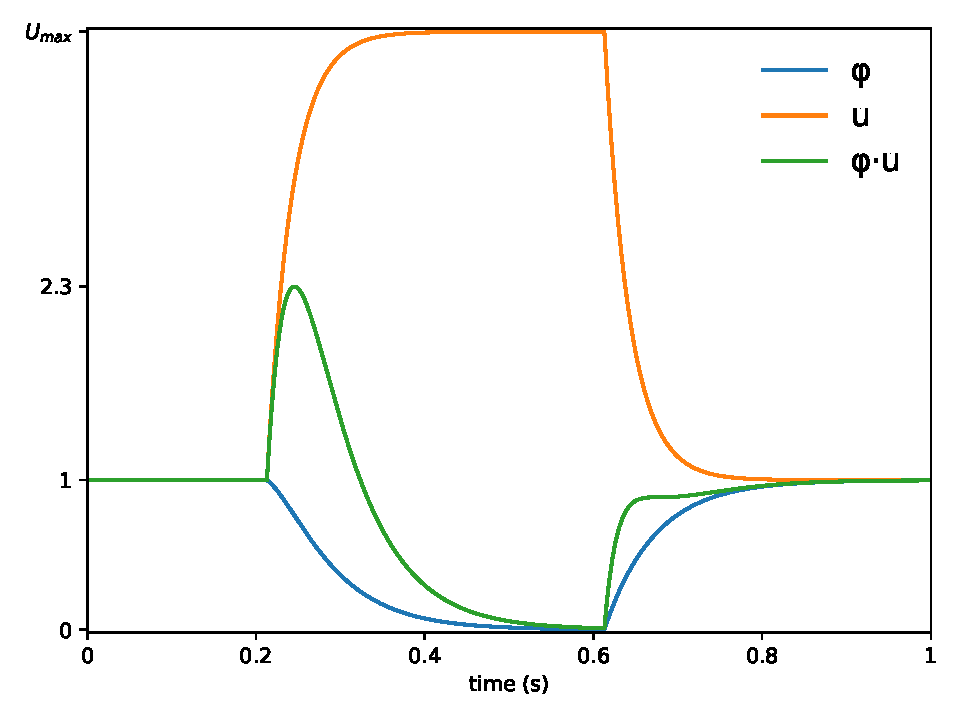
\includegraphics[width=0.7\linewidth]{./full_depletion}
			\caption{Short-term plasticity of a single neuron with high and low input. $T_\varphi=60 \ \text{ms}$, $T_u = 30 \ \text{ms}$}
			\label{fig:full_depletion}
		\end{figure}
		
		These rules can give rise to a transient state dynamics. As an example in a ring with 6 neurons, see Fig. \ref{fig:ring_activity} in which the activation function has a gain of $a=10$.
		
		\begin{figure}
			\centering

			\includegraphics[width=0.7\linewidth]{./ring_activity_g10}
			\includegraphics[width=0.5\linewidth]{./ring}
			\caption{}
			\label{fig:ring_activity}
		\end{figure}
		
		\paragraph{A few words on gains}
		It seems that an appropriately high value of the gain is needed in order to have transient state dynamics instead of a fixpoint, see Fig. \ref{fig:low_gain}, where the neuronal activities for gains $a=1,\ 5$ are shown. It seems that when the gain is too low, the activity does not get close to the extreme of $y = 1$ so the short-term plasticity does not kick in. This problem can be avoided with synaptic weights that are larger in absolute value. 
		
		In fact, consider that the intervals of $x$ in which the sigmoidal goes from $y=0.01$ to $y = 0.99$ for, respectively, gains $a = 1, \ 5, \ 10$ are $\left[-4.6,\ 4.6\right]$, $\left[-0.92,\ 0.92\right]$ and $\left[-0.46,\ 0.46\right]$, while the inputs are effectively restricted to $\left[-2.3,\ 1\right]$, the lower happening when the inhibitory synapses have their maximum efficacy.
		
		Since every neurons behaves the same, for $a=1$ it is possible to compute the steady state activity $y^* \approx 0.2625$ by solving numerically the self-consistent equation for $x_{\text{inp}}^*$:
		\begin{equation}
			x_{\text{inp}}^* = \left(2w_0 + 3 z_0 \varPhi_u^* U_y^* \right) y\left(x_{\text{inp}}^* \right)
		\end{equation}
		
		\begin{figure}
			\includegraphics[width=0.49\linewidth]{./ring_activity_g1}
			\includegraphics[width=0.49\linewidth]{./ring_activity_g5}
			\caption{If the gains are not large enough, the system rapidly goes to a fixpoint.}
			\label{fig:low_gain}
		\end{figure}
		
		\subsection{Learning rule}
		
		
		\newpage
		\printbibliography
\end{document}
